\documentclass[11pt]{article}
\usepackage{cs170}
\usepackage{tikz-qtree}
\usetikzlibrary{arrows}
\usetikzlibrary{shapes}
\usepackage{soul}
\usepackage{xcolor}
\newcommand*\circled[1]{\tikz[baseline=(char.base)]{
            \node[shape=circle,draw,inner sep=2pt] (char) {#1};}}


\def\title{Homework 2}
\def\duedate{Monday 2/5/2024, at 10:00 pm (grace period until 11:59pm)}

\begin{document}
\maketitle
Due \textbf{\duedate}

\question{Study Group}
List the names and SIDs of the members in your study group.
If you have no collaborators, you must explicitly write ``none''.

\begin{solution}
\begin{itemize}
    \item Lakshya Nagal, SID: 3037935253
    \item Joyce Lu, SID: 3039208707
    \item Melad Mayaar, SID: 3038197632
    \item OH and Homework Party
\end{itemize}
\end{solution}

\question{Median}

Recall the \href{https://people.eecs.berkeley.edu/~vazirani/algorithms/chap2.pdf#page=10}{quickselect algorithm} used for quickly finding the median of an array. Suppose you ran quickselect on the following array to find it's median.
\begin{center}
    \begin{tabular}{|c|c|c|c|c|c|c|c|c|c|c|c|}
        \hline
        12 & 78 & 13 & 1 & 97 & 45 & 48 & 26 & 85 & 100 & 78\\ 
        \hline
    \end{tabular}        
\end{center}
\begin{enumerate}

    \item Suppose you always pick the first element as the pivot. List the all the subarrays that quickselect recurses on, as well as the index $k$ -- the $k$ smallest element of the current subarray which the algorithm returns. \\ \\
    For example, quickselect begins on the entire array [12, 78, 13, 1, 97, 45, 48, 26, 85, 100, 78] and $k=6$.\\
    \begin{solution}
        \begin{center}
            \textbf{$1^{st}$ call}\\
            S$_R$ : 
            \begin{tabular}{|c|c|c|c|c|c|c|c|c|c|}
                \hline
                78 & 13 & 97 & 45 & 48 & 26 & 85 & 100 & 78\\ 
                \hline
            \end{tabular}
            , $k = 6$\\
            \textbf{$2^{nd}$ call}\\
            S$_L$ : 
            \begin{tabular}{|c|c|c|c|}
                \hline
                13 & 45 & 48 & 26\\ 
                \hline
            \end{tabular}
            , $k = 4$\\
            \textbf{$3^{rd}$ call}\\
            S$_R$ : 
            \begin{tabular}{|c|c|c|}
                \hline
                45 & 48 & 26\\ 
                \hline
            \end{tabular}
            , $k = 4$\\
            \textbf{$4^{th}$ call}\\
            S$_R$ : 
            \begin{tabular}{|c|}
                \hline
                48\\ 
                \hline
            \end{tabular}
            , $k = 3$ \\
            \textbf{$5^{th}$ call}\\
            $k = 1$, return $\Rightarrow v=48$                                                
        \end{center}
    \end{solution}
    \newpage
    \item Specify which elements should be picked as pivots at each step in order to \textbf{maximize} the runtime of this algorithm. Write the numerical value of the elements, not their indices.\\
    \begin{solution}
        The idea to maximize the runtime would be to chose the smallest or biggest elements as the pivot up to the median number and then pick the opposite of your inital choice (i.e. choose smallest elements as pivots then after median choose largest elements).
        One way would be picking 100, 97, 85, 78, 1, 12, 13, 26, 45, 48, as pivots.
    \end{solution}
    \item Specify which elements should be picked as pivots at each step in order to \textbf{minimize} the runtime of this algorithm. Write the numerical value of the elements, not their indices.\\
    \begin{solution}
        If we pick the median to be our initial pivot then, we return the median immediately after partitioning the input array. 
        We call quickselect on the array above with $k = 6$ and our first pivot is $v = 48$...
        \begin{center}
            S$_L$ : 
            \begin{tabular}{|c|c|c|c|c|}
                \hline
                12 & 13 & 1 & 45 & 26\\ 
                \hline
            \end{tabular} \text{  }
            S$_v$ : 
            \begin{tabular}{|c|}
                \hline
                48\\ 
                \hline
            \end{tabular}  \text{  }
            S$_R$ : 
            \begin{tabular}{|c|c|c|c|c|}
                \hline
                78 & 97 & 85 & 100 & 78\\ 
                \hline
            \end{tabular}
            \begin{align*}
                \left|S_L\right| < k \le \left|S_L\right| + \left|S_v\right| \Rightarrow return \text{ } v = 48
            \end{align*}
        \end{center}
    \end{solution}
\end{enumerate}

\newpage

\question{Median of Medians}

The \textsc{QuickSelect}($A$, $k$) algorithm for finding the $k$th smallest element in an unsorted array $A$ picks an arbitrary pivot, 
then partitions the array into three pieces: the elements less than the pivot, the elements equal to the pivot, and the elements that are greater than the pivot.
It is then recursively called on the piece of the array that still contains the $k$th smallest element.

\begin{subparts}
    \item Consider the array $A = [ 1, 2, \ldots, n]$ shuffled into some arbitrary order. What is the worst-case runtime of \textsc{QuickSelect}($A$, $n/2$) in terms of $n$?
    Construct a sequence of `bad' pivot choices that achieves this worst-case runtime.

    \emph{Hint: refer to Q2.}\\
    \begin{solution}
        A bad pivot would consist of the smallest or largest element of A such as the sequence $1, 2, 3, 4,\dots$. This would yield the runtime:
        \begin{align*}
            n + (n - 1) + (n - 2) + \cdots + \frac{n}{2} = \Theta(n^2)
        \end{align*}
    \end{solution}

\end{subparts}

The above `worst case' has a chance of occurring even with randomly-chosen pivots, so the worst-case time for \textsc{QuickSelect} is $\mathcal{O}(n^2)$, even though it achieves $\Theta(n)$ on average.

    Based on \textsc{QuickSelect}, let's define a new algorithm $\textsc{DeterministicSelect}$ that deterministically picks a consistently good pivot every time.
    This pivot-selection strategy is called `Median of Medians', so that the worst-case runtime of \textsc{DeterministicSelect}($A$, $k$) is $\mathcal{O}(n)$.

\begin{center}
    \begin{minipage}{12cm}
    \begin{framed}
    \noindent\textbf{Median of Medians}

    \begin{enumerate}[1.]
        \item Group the array into $\lfloor n/5 \rfloor$ groups of $5$ elements each (ignore any leftover elements)
        \item Find the median of each group of $5$ elements (as each group has a constant 5 elements, finding each individual median is $\mathcal{O}(1)$)
        \item Create a new array with only the $\lfloor n/5 \rfloor$ medians, and find the true median of this array using \textsc{DeterministicSelect}.
        \item Return this median as the chosen pivot
    \end{enumerate}
    \end{framed}
    \end{minipage}
    \end{center}
    
    \begin{subparts}
    \newpage
    \item[(b)] Let $p$ be the pivot chosen by \textsc{DeterministicSelect} on $A$. Show that at least $3n/10$ elements in $A$ are less than or equal to $p$, and that at least $3n/10$ elements are greater than or equal $p$. \\
        \begin{solution}\\
            Example: \textbf{n = 15} 
            \begin{center}
                \renewcommand{\arraystretch}{1.7}
                $A$: 
                \begin{tabular}{|c|c|c|c|c|c|c|c|c|c|c|c|c|c|c|}
                    \hline
                    92 & 3 & 10 & 26 & 81 & 72 & 5 & 16 & 18 & 23 & 85 & 100 & 12 & 15 & 48 \\
                    \hline
                \end{tabular} \\
                \textbf{Split into $\lfloor \frac{n}{5} \rfloor$ groups: }
                $S_i$ for $0 < i \le \lfloor \frac{n}{5} \rfloor$ \\
                $S_1$:
                \begin{tabular}{|c|c|c|c|c|}
                    \hline
                    92 & 3 & 10 & 26 & 81\\
                    \hline
                \end{tabular}
                $S_2$:
                \begin{tabular}{|c|c|c|c|c|}
                    \hline
                    72 & 5 & 16 & 18 & 23\\
                    \hline
                \end{tabular}
                $S_3$:
                \begin{tabular}{|c|c|c|c|c|}
                    \hline
                    85 & 100 & 12 & 15 & 48 \\
                    \hline
                \end{tabular} \\
                \textbf{Find the median of $S_i$:}\\
                \begin{tabular}{|c|c|c|c|c|}
                    \hline
                    \colorbox{yellow}{3} & \colorbox{yellow}{10} & \color{red}\circled{\textbf{26}} & 81 & 92\\
                    \hline
                \end{tabular}
                \begin{tabular}{|c|c|c|c|c|}
                    \hline
                    \colorbox{yellow}{5} & \colorbox{yellow}{16} & \color{red}\circled{\textbf{18}} & 23 & 72\\
                    \hline
                \end{tabular}
                \begin{tabular}{|c|c|c|c|c|}
                    \hline
                    12 & 15 & \color{red}\circled{\textbf{48}} & 85 & 100 \\
                    \hline
                \end{tabular} \\
                \textbf{Create a new array, $M_f$, with the medians of $S_i$:}\\
                $M_f$: 
                \begin{tabular}{|c|c|c|}
                    \hline
                     26 & 18 & 48 \\
                    \hline
                \end{tabular} \\
                \textbf{Find the median of $M_f$:}\\
                $M_f$: 
                \begin{tabular}{|c|c|c|}
                    \hline
                     18 & \color{red}\circled{\textbf{26}} & 48 \\
                    \hline
                \end{tabular}\\
                Let $m$ denote the median of $M_f$, that is $m = \left\lfloor\frac{|M_f|}{2}\right\rfloor$.
                \renewcommand{\arraystretch}{1.0}
            \end{center}
            $M_f$ contains $\lfloor \frac{n}{5} \rfloor$ elements. To find $m$ we need to retrieve the $\frac{\frac{n}{5}}{2} = \frac{n}{10}$ element.
            We know that every element that comes before $m$ (there are $\frac{n}{10}$ elements) is less than or equal to the $m$. Since we intially grouped 
            $n$ elements into $S_i$ subarrays with five elements in each then found the median of $S_i$, this implies that there are exactly two 
            elements that are less than or equal to the median of $S_i$. Consequently every element 
            from $M_f$ that is less than or equal to $m$ implicitly has two elements that are also less than or equal to $m$. Leaving us with the following equation:
            \begin{align*}
                \frac{n}{10}(2 + 1) = \frac{3n}{10}
            \end{align*}
            where \textbf{$\frac{n}{10}$} is the number of elements to the left of $m$, for which there are \textbf{2} elements in  $S_i$ that are less than or equal to $m$, 
            as well as the elements to the left of $m$ in $M_f$ (\textbf{+1}). By symmetry, the argument for the number of elements that are greater than or equal to $m$ would be the same and yield the same results as above.
        \end{solution}
    \newpage
    \item[(c)] Show that the worst-case runtime of \textsc{DeterministicSelect}($A$, $k$) using the `Median of Medians' strategy is $\mathcal{O}(n)$.
    \textit{Hint: Using the Master theorem will likely not work here. 
    Find a recurrence relation for $T(n)$, and try to use induction to show that $T(n) \leq c \cdot n$ for some $c > 0$.}\\
    \begin{solution}
        Recurrence relation is $T(n) = T(n/5) + T(7n/10) + O(n)$
        \begin{center}
            Now we want to show that $T(n) \le cn, c>0$\\
            \textbf{Base Case: }\\
            The case for small $n$ is trivial, as shown in 3(b) with $n=15$\\
            \textbf{Inductive Hypothesis: }
            \begin{align*}
                T\left(\frac{n}{5}\right) &\le c\left(\frac{n}{5}\right)\\
                T\left(\frac{7n}{10}\right) &\le c\left(\frac{7n}{10}\right)
            \end{align*}
            \textbf{Inductive Step: }
            \begin{align*}
                T(n) &\le c \left(\frac{n}{5}\right) + c\left(\frac{7n}{10}\right) + bn\\
                cn &= c\left(\frac{n}{5}\right) + c\left(\frac{7n}{10}\right) + bn\\
                c &= c\left(\frac{9}{10}\right) + b\\
                c &= 10b
            \end{align*}
        \end{center}
        Thus we have shown that $T(n) \le c\cdot n$ for $c > 0$
    \end{solution}

\end{subparts}

\newpage

\question{The Resistance}

We are playing a variant of The Resistance, a board game where there are $n$ players, $s$ of which are spies. In this variant, in every round, we choose a subset of players to go on a mission. A mission succeeds if the subset of the players does not contain a spy, but fails if at least one spy goes on the mission. After a mission completes, we only know its outcome and not which of the players on the mission were spies.

Come up with a strategy that identifies all the spies in $O(s \log (n/s))$ missions. \textbf{Describe your strategy and analyze the number of missions needed.}

\emph{Hint 1: consider evenly splitting the $n$ players into $x$ disjoint groups (containing $\approx n/x$ players each), and send each group on a mission. At most how many of these $x$ missions can fail? What should you set $x$ to be to ensure that you can reduce your problem by a factor of at least $1/2$?}

\emph{Hint 2: it may help to try a small example like $n=8$ and $s=2$ by hand.}\\
\begin{solution}
    The strategy would be to send the players on a mission, if the mission fails, we split the n players evenly into 2$s$ groups, and recurse on the groups stopping when the mission returns succesful.
    \\ Example: \textbf{n = 8, s = 2 = spy, c $\in$ n, $c \ne s$ with x = 2s = 4}
    \tikzset{every tree node/.style={minimum width=3em,draw,circle},
    blank/.style={draw=none},
    edge from parent/.style=
    {draw,edge from parent path={(\tikzparentnode) -- (\tikzchildnode)}},
    level distance=2.0cm}
    \begin{center}
        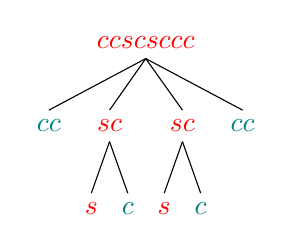
\begin{tikzpicture}
            \Tree
            [.\color{red}$ccscsccc$
                [.\color{teal}$cc$ 
                ]
                [.\color{red}$sc$ 
                \edge[];
                    [.\color{red}$s$
                    ]
                \edge[];
                    [.\color{teal}$c$
                    ]
                ]
                [.\color{red}$sc$ 
                    \edge[];
                        [.\color{red}$s$
                        ]
                    \edge[];
                        [.\color{teal}$c$
                        ]
                ]
                [.\color{teal}$cc$ 
                ]
            ]
        \end{tikzpicture} \\
    \end{center}
    Since at every level at most $s$ missions will fail all the way down to the the $l-1$ level (because at the last l level we know who is a spy and no further missions are needed), 
    and additionallly the height of the tree is $l = \log_{2s}n$ then we have the following relationship:
    \begin{align*}
        s\cdot(l-1) &= s(\log_{2s}n - 1)\\
        &= s(\log_{2s}n - \log_{2s}2s)\\
        &= s(\log_{2s}\left(\frac{n}{2s}\right)\\
        &= s\log\left(\frac{n}{s}\right)
    \end{align*}
    Giving a total runtime of $O(s\log(n/s))$
\end{solution}

\newpage

\question{Among Us}
You are playing a party game with $n$ other friends, who play either as imposters or crewmates.
You do not know who is a crewmate and who is a imposter, but all your friends do.
There are always more crewmates than there are imposters.

Your goal is to identify one player who is certain to be a crewmate.

Your allowed `query' operation is as follows: you pick two players as partners. You ask each player if their partner is a crewmate or a imposter.
When you do this, a crewmate must tell the truth about the identity of their partner,
but a imposter doesn't have to (they may lie or tell the truth about their partner).

Your algorithm should work regardless of the behavior of the imposters.

\begin{subparts}
	\subpart For a given player $x$, devise an algorithm that returns whether or not $x$ is a crewmate using $O(n)$ queries. Just an informal description of your test and a brief explanation of why it works is needed.\\
    \begin{solution}
        The simplest solution would be to take a vote from the $n-1$ players and go with the popular vote. This is guaranteed
        to expose player $x$ since the majority of the $n-1$ players are crewmates who can only tell the truth. This would yield a time complexity 
        of $O(n)$ since at most you have ask $n$. 
    \end{solution}
    \newpage
	\subpart Show how to find a crewmate in $O(n\log n)$ queries (where one query is taking two players $x$ and $y$ and asking $x$ to identify $y$ and $y$ to identify $x$).
	\textit{Hint: Split the players into two groups, recurse on each group, and use part (a). What invariant must hold for at least one of the two groups?}

	\textbf{Give a \href{https://cs170.org/resources/homework-guidelines/}{3-part solution}.}\\
    \begin{solution}\\
        \tikzset{every tree node/.style={minimum width=2em,draw,circle},
        blank/.style={draw=none},
        edge from parent/.style=
        {draw,edge from parent path={(\tikzparentnode) -- (\tikzchildnode)}},
        level distance=1.2cm}
        \begin{center}
            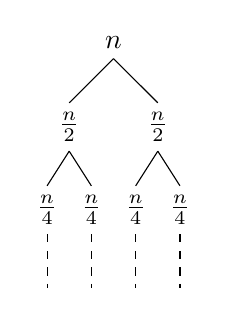
\begin{tikzpicture}
                \Tree
                [.$n$
                    [.$\frac{n}{2}$ 
                        \edge[];
                        [.$\frac{n}{4}$
                            \edge[dashed];
                            [.$$
                            ]
                        ]
                        \edge[];
                        [.$\frac{n}{4}$
                            \edge[dashed];
                            [.$$
                            ]
                        ]
                    ]
                    [.$\frac{n}{2}$ 
                        \edge[];
                        [.$\frac{n}{4}$
                            \edge[dashed];
                            [.$$
                            ]
                        ]
                        \edge[];
                        [.$\frac{n}{4}$
                            \edge[dashed];
                            [.$$
                            ]
                        ]
                    ]
                ]
            \end{tikzpicture} \\
        \end{center}
        \textbf{Algorithm Description: }\\
        We split the players into two groups and keep splitting until there are around 3 players in each group. At which point we can run 
        the algorithm from part (a) and keep only the players that are voted as being crewmates by the majority of the group. \\
        \textbf{Proof of Correctness: }\\
        \begin{center}
            \textbf{Inductive Hypothesis: }\\
            The algorithm above indentifies a crewmate amongst n players or less.\\
            \textbf{Base Case: n$\le$ 3}\\
            From the description of the game, we know there are more players than imposter, so the majority vote should suffice to find a crewmate.\\
            \textbf{Inductive Step: }\\
            From our inductive hypothesis we know that the algorithm works for groups with less than or equal to 3 players.
            Since we recursively keep splitting the n players into 2 groups until we are eventually left with a finite number of players in each group.
            From our base case we know that the algorithm in part (a) can identify a crewmate, so keep on those players.
        \end{center}
        \textbf{Runtime Analysis: }\\
        The above algorithm gives the following recurrence relation: $T(n) = 2T(\frac{n}{2}) + O(n)$. From the tree abovewe can
        see our branching factor is 2. The total amount of work done is $\sum_{k = 0}^{\log_2n}2^k\frac{n}{2^k} = n\sum_{k = 0}^{\log_2n}1 = O(n\log n)$
    \end{solution}
\end{subparts}
\newpage
\question{Modular Fourier Transform}
Fourier transforms (FT) have to deal with computations involving irrational numbers which can be tricky to implement in practice.
Motivated by this, in this problem you will demonstrate how to do a Fourier transform in modular arithmetic,
using modulo 5 as an example.
\begin{subparts}
\subpart There exists $\omega \in \{0, 1, 2, 3, 4\}$ such that $\{\omega^0, \omega^1, \omega^2, \omega^3\}$ the are $4^{th}$ roots of unity (modulo 5), i.e., solutions to $z^4 = 1 \pmod 5$. When doing the FT in modulo 5, this $\omega$ will serve a similar role to the primitive root of unity in our standard FT. Show that $\{1,2,3,4\}$ are the $4^{th}$ roots of unity (modulo 5), with $\omega=2$ as the primitive root. Also show that $1+\omega + \omega^2 + \omega^3 = 0 \pmod 5$ for $\omega=2$.\\
\begin{solution}\\
    \begin{align*}
        1^4 &= 1 \equiv 1\text{ (mod } 5)\\
        2^4 &= 16 \equiv 1\text{ (mod } 5)\\
        3^4 &= 81 \equiv 1\text{ (mod } 5)\\
        4^4 &= 256 \equiv 1\text{ (mod } 5)
    \end{align*}
    \begin{center}
        Since $\left(1, 2, 3, 4\right)$ raised to the $4^{th}$ gives back $1$, $(1, 2, 3, 4)$ are the $4^{th}$ \\roots of unity (modulo $5$).
    \end{center}
    \begin{align*}
        2^0 = 1 &\equiv 1\text{ (mod } 5)\\
        2^1 = 2 &\equiv 2\text{ (mod } 5)\\
        2^2 = 4 &\equiv 4\text{ (mod } 5)\\
        2^3 = 8 &\equiv 3\text{ (mod } 5)\\
        2^4 = 16 &\equiv 1\text{ (mod } 5)\\
        2^5 = 32 &\equiv 2\text{ (mod } 5)\\
        2^6 = 64 &\equiv 4\text{ (mod } 5)\\
        2^7 = 128 &\equiv 3\text{ (mod } 5)\\
        &\vdots\\
        1+\omega + \omega^2 + \omega^3 = 1 + &2 + 4 + 3 = 10 \equiv 0\text{ (mod } 5)
    \end{align*}
\end{solution}
\newpage
\subpart Using the FFT, produce the transform of the sequence $(0, 2, 3, 0)$ modulo 5; that is, evaluate the polynomial $2x+3x^2$ at $\{1, 2, 4, 3\}$ using the recursive FFT algorithm defined in class, but with $\omega=2$ and in modulo 5 instead of with $\omega=i$ in the complex numbers. Note that all calculations should be performed modulo 5. 

\textit{Hint: You can verify your calculation by evaluating the polynomial at $\{1, 2, 4, 3\}$ using the slow method (i.e. DFT).}\\
\begin{solution}
    \begin{align*}
       FFT(&[0, 2, 3, 2], [1, 3, 4, 2])\\
        &E_0(x) = 0 + 3x\\
        &\begin{aligned}
            FFT(&[0, 3], [1, 4])\\
            &E_1(x) = 0 \hookrightarrow 0\\
            &O_1(x) = 3 \hookrightarrow 3\\
            \hookrightarrow &P(1) = E_1(1^2) + 1 \cdot O_1(1^2) = 0 + 3 = 3 \equiv 3 \pmod5\\
            \hookrightarrow &P(4) = E_1(4^2) + 4 \cdot O_1(4^2) = 0 + 12 = 12 \equiv 2 \pmod5\\
        \end{aligned} \\
        &O_0(x) = 2 + 0x\\
        &\begin{aligned}
            FFT(&[2, 0], [1, 4])\\
            &E_1(x) = 2 \hookrightarrow 2\\
            &O_1(x) = 0 \hookrightarrow 0\\
            \hookrightarrow &P(1) = E_1(1^2) + 1 \cdot O_1(1^2) = 2 + 0 = 2 \equiv 2 \pmod5\\
            \hookrightarrow &P(4) = E_1(4^2) + 4 \cdot O_1(4^2) = 2 + 0 = 2 \equiv 2 \pmod5\\
        \end{aligned} \\
        \hookrightarrow &P(1) = E(1^2) + 1 \cdot O(1^2) = 3 + 2 = 5 \equiv 0 \pmod5\\
        \hookrightarrow &P(2) = E(2^2) + 2 \cdot O(2^2) = 2 + 4 = 6 \equiv 1 \pmod5\\
        \hookrightarrow &P(4) = E(4^2) + 4 \cdot O(4^2) = 3 + 8 = 11 \equiv 1 \pmod5\\
        \hookrightarrow &P(3) = E(3^2) + 3 \cdot O(3^2) = 2 + 6 = 8 \equiv 3 \pmod5\\
        \Rightarrow &\textbf{return }\boxed{[0, 1, 1, 3}
    \end{align*}
\end{solution}
\newpage
\subpart Now perform the inverse FFT on the sequence $(0, 1, 4, 0)$, also using the recursive algorithm. Recall that the inverse FFT is the same as the forward FFT, but using $\omega^{-1}$ instead of $\omega$, and with an extra multiplication by $4^{-1}$ for normalization.\\
\begin{solution}\\
    Inverses: [1, 3, 4, 2]
    \begin{align*}
       FFT(&[0, 1, 4, 0], [1, 3, 4, 2])\\
        &E_0(x) = 0 + 4x\\
        &\begin{aligned}
            FFT(&[0, 4], [1, 4])\\
            &E_1(x) = 0 \hookrightarrow 0\\
            &O_1(x) = 4 \hookrightarrow 4\\
            \hookrightarrow &P(1) = E_1(1^2) + 1 \cdot O_1(1^2) = 0 + 4 = 4 \equiv 4 \pmod5\\
            \hookrightarrow &P(4) = E_1(4^2) + 4 \cdot O_1(4^2) = 0 + 16 = 16 \equiv 1 \pmod5\\
        \end{aligned} \\
        &O_0(x) = 1 + 0x\\
        &\begin{aligned}
            FFT(&[1, 0], [1, 4])\\
            &E_1(x) = 1 \hookrightarrow 1\\
            &O_1(x) = 0 \hookrightarrow 0\\
            \hookrightarrow &P(1) = E_1(1^2) + 1 \cdot O_1(1^2) = 1 + 0 = 1 \equiv 1 \pmod5\\
            \hookrightarrow &P(4) = E_1(4^2) + 4 \cdot O_1(4^2) = 1 + 0 = 1 \equiv 1 \pmod5\\
        \end{aligned} \\
        \hookrightarrow &P(1) = E(1^2) + 1 \cdot O(1^2) = 4 + 1 = 5 \equiv 0 \pmod5\\
        \hookrightarrow &P(3) = E(3^2) + 3 \cdot O(3^2) = 16 + 3 = 19 \equiv 4 \pmod5\\
        \hookrightarrow &P(4) = E(4^2) + 4 \cdot O(4^2) = 4 + 4 = 8 \equiv 3 \pmod5\\
        \hookrightarrow &P(2) = E(2^2) + 2 \cdot O(2^2) = 16 + 2 = 18 \equiv 3 \pmod5\\
        \Rightarrow &\textbf{return }4\cdot[0, 4, 3, 3] = [0, 16, 12, 12] = \boxed{[0, 1, 2, 2] \pmod 5}
    \end{align*}
\end{solution}
\subpart Now show how to multiply the polynomials $2x + 3x^2$ and $3 - x$ using the FFT modulo 5. You may use the fact that the FFT of $(3, 4, 0, 0)$ modulo 5 is $(2, 1, 4, 0)$ without doing your own calculation.\\
\begin{solution}\\
    First we calculat ethe FFT of $2x + 3x^2$ and $3 - x$ (modulo 5) with the $4^{th}$ roots of unity from part (a). From part (b) we know that 
    the FFT of $2x + 3x^2 = [0, 1, 1, 3]$. The FFT of $3 - x$ was given as $[2, 1, 4, 0]$. We know multiply the two vectors point wise resulting in 
    $[0, 1, 4, 0]$. We then find the inverse of $0 + x + 4x^2 + 0x^3 \Rightarrow [0, 1, 4, 0]$ which we found in part (c) to get the final polynomial.
\end{solution}
\end{subparts}
\end{document}